\documentclass[10pt]{article}

\PassOptionsToPackage{hidelinks}{hyperref}
\usepackage[utf8]{inputenc}
\usepackage{amsmath, calc, xcolor}
\usepackage{alphabeta} 
\usepackage[pdftex]{graphicx}
\usepackage[top=1in, bottom=1in, left=1in, right=1in]{geometry}
\usepackage[]{bookmark}
\linespread{1.06}
\setlength{\parskip}{8pt plus2pt minus2pt}

\widowpenalty 10000
\clubpenalty 10000

\newcommand{\eat}[1]{}
\newcommand{\HRule}{\rule{\linewidth}{0.5mm}}
\usepackage[official]{eurosym}
\usepackage{enumitem}
\setlist{nolistsep,noitemsep}
\usepackage[]{hyperref}
\usepackage{url}
\usepackage{cite}
\usepackage{lipsum}
\usepackage{indentfirst}
\usepackage{tikz}
\usetikzlibrary{arrows,decorations.pathmorphing,backgrounds,fit,positioning,shapes.symbols,chains}
\usepackage{xcolor,colortbl}
\usepackage{array}

\setlength{\parindent}{2em}
\renewcommand*\contentsname{Índice}
\renewcommand\refname{}

\begin{document}

%===========================================================
\begin{titlepage}
\begin{center}

% Top 

\includegraphics[width=0.55\textwidth]{img/logo-isec-transparente.png}~\\[2cm]


% Title
\HRule \\[0.4cm]
{ \LARGE 
  \textbf{Inteligência Computacional}\\[0.4cm]
}
\HRule \\[1.5cm]

% Docente
{ \large
  \textbf{Docente} \\[0.1cm]
  Inês Dominguês \\ Carlos Pereira \\[2.5cm]
}


% Author
{ \large
  \textbf{Alunos} \\[0.1cm]
  Paulo Henrique Figueira Pestana de Gouveia - a2020121705 \\[0.1cm]
  Nuno Alexandre Almeida Santos - a2019110035\\[0.1cm]
}

\vfill



% Bottom
{\large \today}
 
\end{center}
\end{titlepage}


\newpage



%===========================================================
\tableofcontents
\addtocontents{toc}{\protect\thispagestyle{empty}}
\newpage
\setcounter{page}{1}

%===========================================================
%===========================================================
\large
\section{Descrição do Problema}\label{sec:intro}
Enfrentamos um problema de regressão em que nosso objetivo é treinar 
uma rede densa e uma rede de convolução de uma dimensão 
para estimar o valor do Bitcoin a cada minuto. 

Sabemos que não será possível estimar o valor exato do Bitcoin, 
pois existem fatores externos que não podemos controlar ou prever 
(como Elon Musk e outros influenciadores), mas nosso objetivo é ficar 
o mais próximo possível. 

Dado que nossa rede será treinada com exemplos de 1/01/2021 a 12/05/2021, 
após o treinamento da rede, compararemos nossos valores obtidos 
com os valores reais nos dias após o último dia em que a rede foi treinada. 

Inicialmente, a escolha dos hiperparâmetros é feita manualmente, realizamos 
vários testes com diferentes variações, analisando o impacto de cada um 
na performance. 

Em seguida, utilizaremos a técnica de "GridSearch" para escolher os melhores valores 
para os hiperparâmetros e o algoritmo PSO para explorar iterativamente o espaço de pesquisa 
e encontrar a solução ótima, otimizando também os hiperparâmetros.

Compararemos ambas as metodologias fazendo uma análise das suas diferenças
e qual teve a melhor performance.

\section{Descrição das Metodologias}\label{sec:desc-das-met}
\subsection{Metodologias Comum em ambas as fases}

O ficheiro CSV "main.csv" é lido e armazenado em um conjunto de dados, 
que é dividido em um conjunto de treinamento que contém 80\% dos dados
e um conjunto de teste com o resto.

O conjunto de dados é pré-processado usando o MinMaxScaler 
para garantir que todas as colunas tenham valores entre 0 e 1.

\subsection{Metodologias Manual}

Uma rede neural é criada usando o TensorFlow. 
A rede é composta por uma camada de entrada, 
seguida por camadas ocultas de neurônios e uma camada de saída.

A quantidade de camadas, neurônios, as funções de ativação usadas variávam
conforme eram variados os testes.

Em seguida, o modelo é compilado usando um otimizador com um "learning rate"
que também era variado, e uma função de perda "binary\_crossentropy",
pois estamos lidando com um problema de classificação binária 
(prever se o valor do Bitcoin aumentará ou diminuirá).

Após compilar o modelo, ele é treinado usando o método fit() do TensorFlow. 
O conjunto de treinamento e as etiquetas de treinamento 
são passados como argumentos para o método. Algumas configurações adicionais 
também são especificadas, como o número de épocas 
(iterações através do conjunto de treinamento) e o tamanho do batch 
(quantas amostras são usadas em cada atualização dos pesos da rede).

Durante o treinamento, o modelo ajusta seus pesos e biases para minimizar 
a função de perda. Isso é feito usando o algoritmo de otimização Adam, 
que atualiza os pesos da rede a cada lote usando uma combinação de 
gradiente descendente estocástico e momentum.

Após o treinamento, o modelo é avaliado usando o conjunto de teste 
e as etiquetas de teste correspondentes. O método evaluate() do TensorFlow 
é usado para calcular a precisão do modelo. A precisão é medida como a 
percentagem de previsões corretas feitas pelo modelo.

Finalmente, as previsões são feitas usando o método predict() do TensorFlow. 
O conjunto de teste é passado como argumento para o método e as previsões 
são armazenadas em uma variável.

Por fim, o modelo é salvo em um arquivo para que possa ser usado 
posteriormente. Isso é feito usando o método save() do TensorFlow.

\subsection{Metodologia GridSearch}
Esta é uma implementação de procura em grelha (grid search) para otimizar 
os hiperparâmetros de um modelo de regressão de redes neurais (MLPRegressor). 
A procura em grelha é uma técnica que consiste em testar todas as combinações 
possíveis de valores de hiperparâmetros especificados num dicionário 
de parâmetros (parameters).

O dicionário de parâmetros em causa inclui duas chaves:
\begin{itemize}
  \item 'hidden\_layer\_sizes'
  \item 'activation'
\end{itemize} 

A chave 'hidden\_layer\_sizes' especifica uma lista de tuplos, 
onde cada tuplo representa uma configuração de tamanho de camadas escondidas
para testar. A chave 'activation' especifica uma lista de funções de ativação 
para testar.

O objeto GridSearchCV é inicializado com um modelo 
MLPRegressor e os parâmetros especificados no dicionário 'parameters', 
além de outros parâmetros. O parâmetro 'scoring' especifica a métrica usada 
para avaliar os modelos durante a procura em grelha. O parâmetro 'n\_jobs' 
especifica o número de processadores a serem usados na procura em 
grelha (-1 significa usar todos os processadores disponíveis). 
O parâmetro 'cv' especifica o número de dobras para usar na validação cruzada.

Por fim, o método 'fit' é usado para treinar o modelo com o conjunto de 
treino 'normed\_train\_dataset' e as etiquetas de treino 'train\_labels'. Isso 
executa a procura em grelha e treina e avalia modelos para cada combinação de 
hiperparâmetros especificados. O modelo com os melhores hiperparâmetros é 
armazenado internamente no objeto GridSearchCV.

\newpage

\subsection{Metodologia Pso}
Nesta função, a metodologia usada é a Otimização por Enxame de Partículas 
(Particle Swarm Optimization, PSO). O objetivo é encontrar os parâmetros 
ótimos de um modelo de redes neurais (definido na função "objective") através 
do uso de uma abordagem de otimização baseada em metaheurísticas.

O algoritmo de PSO é inicializado com uma função "optimizer" que define 
alguns parâmetros de configuração, como o número de partículas (n\_particles),
o número de dimensões (dimensions) e os coeficientes c1 e c2. Também é 
especificado um conjunto de limites (bounds) para os parâmetros a serem 
otimizados.

A função "f" é usada como a função objetivo para otimizar. Ela itera sobre um 
conjunto de entradas (x) e avalia a função "objective" para cada uma dessas 
entradas. A função "objective" constrói um modelo de redes neurais com base 
nos parâmetros de entrada e, em seguida, treina esse modelo com os dados de 
treinamento e retorna uma medida de perda (loss). A função "f" retorna um 
vetor de perdas para cada uma das entradas.

O algoritmo de PSO é então executado por um número especificado de 
iterações (iters) usando a função "optimize", com o objetivo de minimizar a 
função "f". No final, são retornados os parâmetros ótimos (xopt) e o valor 
mínimo da função (fopt).

\section{Implementação dos Algoritmo}\label{sec:imp-al}

O algoritmo de Otimização por Enxame de Partículas 
(Particle Swarm Optimization, PSO) é uma técnica de otimização baseada em 
metaheurísticas que imita o comportamento de um enxame de partículas em 
movimento. É usado para encontrar o mínimo ou máximo de uma função objetivo 
em um conjunto de parâmetros.

A implementação neste código começa com a definição de duas funções, 
"f" e "objective". A função "f" é usada como a função objetivo para o 
algoritmo de PSO. Ela itera sobre um conjunto de entradas (x) e avalia a 
função "objective" para cada uma dessas entradas. A função "objective" 
extrai os hiperparâmetros das entradas (hidden\_layer\_sizes) e usa esses 
hiperparâmetros para construir um modelo de redes neurais usando o framework 
Keras. Em seguida, o modelo é compilado e treinado com os dados de 
treinamento e uma medida de perda (loss) é calculada como a média da perda ao 
longo de todas as épocas de treinamento. Essa perda é então retornada pela 
função "objective". A função "f" retorna um vetor de perdas para cada uma das 
entradas.

Em seguida, é criado o otimizador de PSO com alguns parâmetros de configuração,
incluindo o número de partículas (n\_particles), o número de dimensões 
(dimensions) e os coeficientes c1 e c2. Também é especificado um conjunto de 
limites (bounds) para os parâmetros a serem otimizados.

Por fim, o algoritmo de PSO é executado por um número especificado de 
iterações (iters) usando a função "optimize", com o objetivo de minimizar a 
função "f". No final, são retornados os parâmetros ótimos (xopt) e o valor 
mínimo da função (fopt).

Além disso, há também uma variável global "best\_model" que é 
atualizada com o modelo de redes neurais que obteve a menor perda ao longo 
do processo de otimização. Além disso, há uma variável global "best\_score" 
que armazena o valor da menor perda encontrada até o momento. Essas variáveis 
podem ser usadas para acessar o modelo e o resultado final da otimização após 
o término do processo.

\section{Análise dos Resultados}\label{sec:anal-res}
\subsection{Parte Manual}
\subsubsection{Deep Network}
Uma rede densa é uma rede neural em que todos os neurônios em uma camada são 
conectados a todos os neurônios na camada seguinte. Ou seja, as camadas da 
rede são completamente "densas", ou seja, não há nenhum neurônio 
"desconectado" ou sem saída.

Iniciamos a análise dos resultados obtidos com as redes densas do Keras, 
onde os parâmetros eram ajustados manualmente após cada teste.

Como rede base para comparação temos:

\begin{figure}[htb]
  \centering
  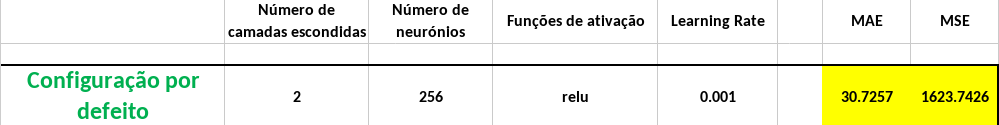
\includegraphics[width=\linewidth]{img/deep_default.png}
  \caption{Rede Densa Default}
  \label{fig:deep_default}
\end{figure}

\newpage
Os primeiros parâmetros que foram alterados foram a quantidade de 
camadas e de neurônios em cada camada.
A quantidade de camadas e de neurônios em cada camada de uma rede neural é 
um hiperparâmetro importante que pode afetar a capacidade da rede de aprender 
padrões nos dados de treinamento.

\begin{figure}[htb]
  \centering
  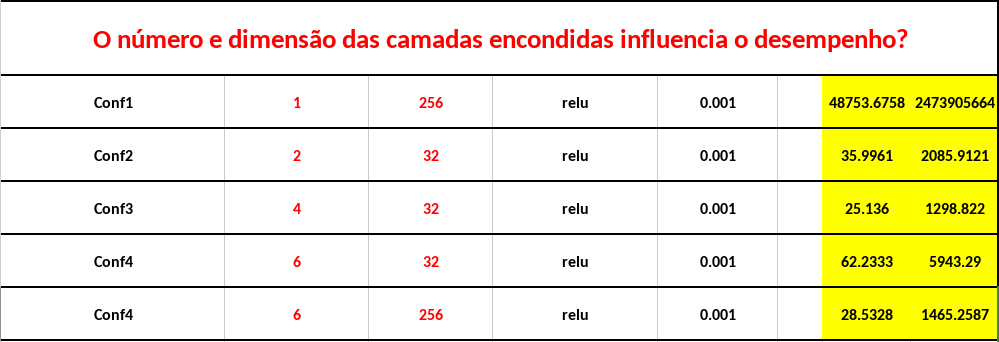
\includegraphics[width=\linewidth]{img/deep_camadas_neuronios.png}
  \caption{Rede Densa com Camadas e Neurônios alterados}
  \label{fig:deep_camadas_neuronios}
\end{figure}

Analisando esta tabela, observamos que a rede obteve melhores 
resultados com 4 camadas e 32 neurônios em cada uma delas. Isso faz sentido, 
pois essa configuração não é tão elevada a ponto de correr o risco de 
overfitting, mas também não é tão baixa que a rede teria dificuldade 
em detetar padrões.

\vspace{1cm}

Proxímo parametro a ser alterado é o learning rate, é um parâmetro utilizado 
em algoritmos de aprendizado de máquina que determina a velocidade com que 
os pesos da rede são atualizados durante o treinamento.

\begin{figure}[htb]
  \centering
  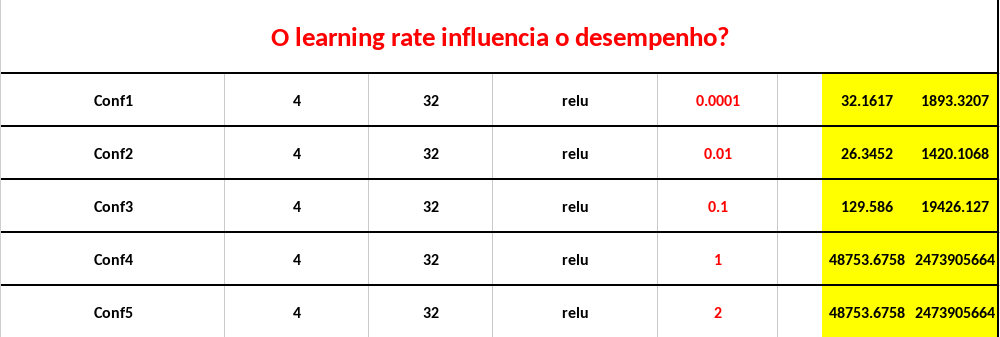
\includegraphics[width=\linewidth]{img/deep_lr.png}
  \caption{Rede Densa com Learning Rate alterado}
  \label{fig:deep_lr}
\end{figure}

Como podemos concluir, o learning rate ideal continua a ser 0.001,
se o learning rate for muito pequeno, o treinamento pode levar muito 
tempo para convergir, enquanto um learning rate muito alto pode fazer 
com que o treinamento não converja ou oscile em torno do ótimo.

\newpage
Por último variamos as funções de ativação da rede, algumas funções de 
ativação podem ser mais adequadas para certos tipos de problemas ou dados, 
enquanto outras podem ser menos eficientes. Além disso, a escolha da função 
de ativação pode afetar a velocidade do treinamento e a capacidade da rede 
de generalizar para novos dados.

\begin{figure}[htb]
  \centering
  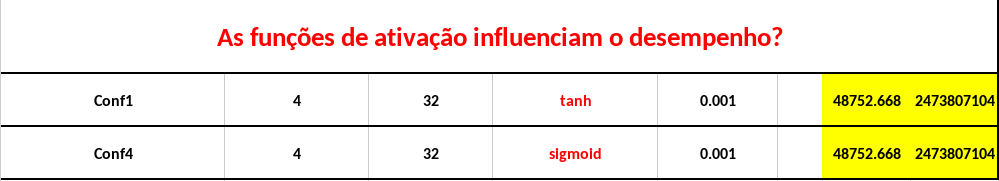
\includegraphics[width=\linewidth]{img/deep_ativacao.png}
  \caption{Rede Densa com funções de ativação alteradas}
  \label{fig:deep_ativacao}
\end{figure}

Conforme podemos observar, os resultados foram os mesmos independentemente 
da função de ativação utilizada, o que indica que a rede não aprendeu nada 
com elas. Isso foi inesperado, pois os dados estavam normalizados entre 0 e 1 
e esperávamos que a sigmóide produzisse bons resultados, mas isso não ocorreu.

A sigmóide pode estar sofrendo do problema do "gradiente desaparecimento", 
onde o gradiente da função torna-se muito pequeno, o que dificulta o 
treinamento da rede. Isso pode ser corrigido utilizando outra função de 
ativação ou ajustando o learning rate.

\subsubsection{CNN 1D}
Uma CNN (rede neural convolucional) 1D é uma rede neural utilizada 
para processar sinais unidimensionais, como séries temporais ou áudio. Ela 
é semelhante às redes densas, mas possui camadas de filtros que são aplicadas 
de forma deslizante (convolucional) ao sinal de entrada.

As camadas de filtros da CNN 1D são compostas por filtros que são aplicados a 
janelas do sinal de entrada e são treinados para extrair características 
relevantes do sinal. Essas características são então passadas para camadas 
densas para a classificação ou a predição final.

Iniciamos a análise dos resultados obtidos com as redes CNN 1D do Keras, 
onde os parâmetros eram ajustados manualmente após cada teste.

\newpage
Como rede base para comparação temos:

\begin{figure}[htb]
  \centering
  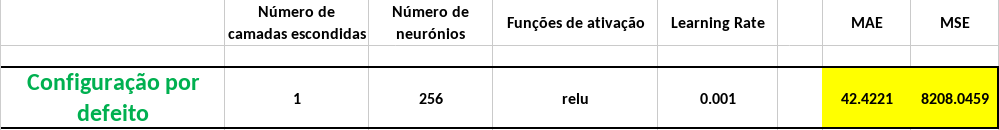
\includegraphics[width=\linewidth]{img/cnn_default.png}
  \caption{Rede CNN 1D Default}
  \label{fig:cnn_default}
\end{figure}

\vspace{1cm}
Os primeiros parâmetros que foram alterados foram a quantidade de 
camadas e de neurônios em cada camada.

\begin{figure}[htb]
  \centering
  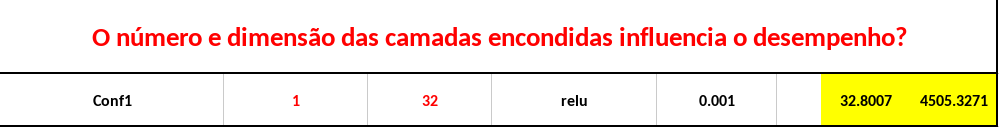
\includegraphics[width=\linewidth]{img/cnn_neuronios.png}
  \caption{Rede CNN 1D neurônios alterados}
  \label{fig:cnn_neuronios}
\end{figure}

Reparamos que aconteceu algo semelhante nas redes densas, que menos neurônios
resultou num erro menor. As CNNs 1D podem se beneficiar de um número menor 
de neurônios em algumas situações, mas isso depende do problema específico 
e da estrutura da rede. Em geral, uma rede com menos neurônios pode ser mais 
fácil de treinar e ter menor risco de overfitting, pois há menos parâmetros 
para ajustar.

\vspace{1cm}
Proxímo parametro a ser alterado é o learning rate, é um parâmetro utilizado 
em algoritmos de aprendizado de máquina que determina a velocidade com que 
os pesos da rede são atualizados durante o treinamento.

\begin{figure}[htb]
  \centering
  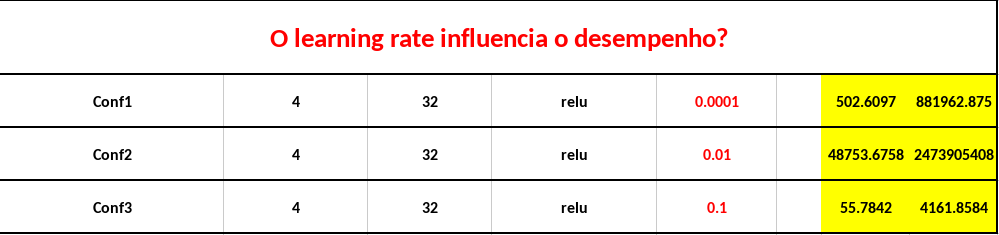
\includegraphics[width=\linewidth]{img/cnn_lr.png}
  \caption{Rede CNN 1D Learning Rate Alterado}
  \label{fig:cnn_lr}
\end{figure}

Neste caso, observamos que a rede de convolução 1D se beneficiou de um 
learning rate mais alto, o que significa que ajudou a convergir mais 
rapidamente para a solução ótima durante o ajuste dos pesos.

\newpage
Por último variamos as funções de ativação da rede, algumas funções de 
ativação podem ser mais adequadas para certos tipos de problemas ou dados, 
enquanto outras podem ser menos eficientes.

\begin{figure}[htb]
  \centering
  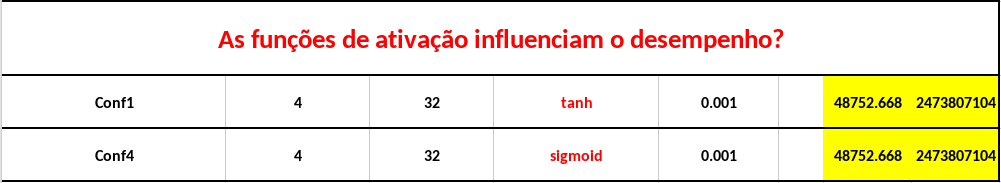
\includegraphics[width=\linewidth]{img/cnn_ativacao.png}
  \caption{Rede CNN 1D Learning Rate Alterado}
  \label{fig:cnn_ativacao}
\end{figure}

Da mesma forma que ocorreu nas redes densas, as funções de ativação testadas aqui não 
conseguiram convergir para a solução ótima.

\subsection{GridSearch}
Como antes referido, o GridSearch é uma técnica que consiste em testar todas as combinações 
possíveis de valores de hiperparâmetros especificados num dicionário de parâmetros.

Decidimos variar os hiperparâmetros camadas,neurônios e funções de ativação:

\begin{figure}[htb]
  \begin{verbatim}
    bounds = [(32, 128), (1, 4)]
    parameters = {
    'hidden_layer_sizes': [(128,), (32,), (32,32), (128,128)],
    'activation': ['tanh','relu','softmax'],
    }
  \end{verbatim}
  \caption{Code block}
  \label{fig:code_1}
\end{figure}

\begin{verbatim}
  
\end{verbatim}

\newpage
O modelo de aprendizagem usado foi MLPRegressor(), pois este é um problema de regressão. 
Foi utilizado 5 folds na validação cruzada e a melhor combinação foi encontrada com o seu 
respectivo erro:

\begin{figure}[htb]
  \centering
  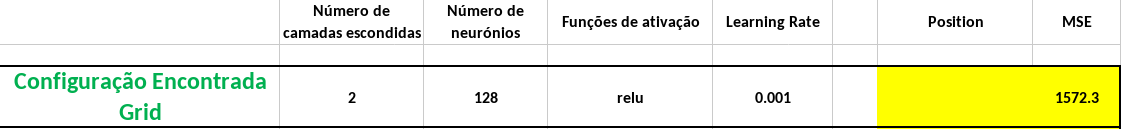
\includegraphics[width=\linewidth]{img/grid.png}
  \caption{Melhor rede dada pelos GridSearch}
  \label{fig:grid}
\end{figure}

O resultado obtido foi pior do que redes anteriores, como a rede densa de 4 camadas e 
32 neurônios em cada uma. Isso é esperado, pois devido ao GridSearch levar muito tempo para 
testar as combinações de hiperparâmetros, decidimos não incluir muitas opções para não exceder 
o limite do nosso hardware e do tempo disponível. Além disso, o código não utiliza uma GPU para 
acelerar o treinamento da rede.

\subsection{PSO}

Utilizamos a mesma abordagem para o PSO, fornecendo limites de busca (bounds) para o 
algoritmo, especificando o número de partículas a serem utilizadas, definindo a dimensão do 
espaço de busca e fornecendo um dicionário de opções para o PSO:

\begin{figure}[htb]
  \begin{verbatim}
    bounds = [(32, 128), (1, 4)]
    # Create the PSO optimizer
    options = {'c1': 0.5, 'c2': 0.3, 'w':1.5}
    optimizer = ps.single.GlobalBestPSO(n_particles=5, dimensions=2, options=options,bounds=bounds)
  \end{verbatim}
  \caption{Code block}
  \label{fig:code_2}
\end{figure}

Em seguida, utilizamos as funções criadas para otimizar os hiperparâmetros e obtivemos 
a seguinte configuração:

\newpage
\section{Conclusão}\label{sec:conc}

Neste trabalho, aprendemos sobre o que são redes densas e redes de convulsão, 
e como elas diferem quando criamos uma rede. Também percebemos o quão trabalhoso é 
otimizar manualmente e variar os hiperparâmetros para obter o menor erro possível.

O PSO, um algoritmo de otimização metaheurístico que imita o comportamento 
de um enxame de partículas em busca do ótimo global de uma função. Utiliza uma estratégia de 
busca heurística e faz suposições sobre a estrutura da função que está sendo otimizada. 

Por outro lado, o GridSearch é um algoritmo de busca exaustiva que pesquisa extensivamente 
um espaço de parâmetros especificado em busca da melhor combinação de valores de hiperparâmetros. Ele não utiliza nenhuma heurística ou faz suposições sobre a estrutura da função, e é garantido que encontrará o ótimo global se o espaço de pesquisa for suficientemente pequeno e o tempo de computação for suficiente. Em contraste, o PSO não garante encontrar o ótimo global, mas pode muitas vezes encontrar soluções boas rapidamente e com relativamente poucas avaliações da função.

Ambos os algoritmos são úteis para criar e treinar redes para encontrar os melhores 
hiperparâmetros, tudo depende do hardware disponível e do objetivo do problema.

\section{Referências}\label{sec:sup-inf-utl}
\bibliographystyle{ieeetr}
\bibliography{refs}


%===========================================================

%===========================================================

\pagebreak
\end{document} 
